\subsection{Time Difference of Arrival}
\label{subsec:03_tdoa}

The \ac{TDOA} estimation is the main component to identify the
whistle source location.
Theoretical background to this approach of source localization is
given in \cref{sec:02_tdoa}.
As stated there, the \ac{TDOA} of a signal measured between two microphone sensors
provides details about the direction of the source.
Having four channels attached on a NAO's head, an overdetermined system it
given where each channel pair provides \ac{TDOA} information.

The \ac{GCC-PHAT} method is a modification of the \ac{CC} method.
Due to their implementation being equal except of the weighting function,
they are discussed in \cref{subsubsec:03_cc} collectively.
\Cref{subsubsec:03_phase} presents the implementation details with its
circumstances.
% -------------------------------------------------------------

\subsubsection{Correlation}
\label{subsubsec:03_cc}

In theory, \acf{CC} in time domain is usually illustrated by shifting
two signals over each other and recording the similarity for each shift.
Similarity in terms of signal processing is measured by the area under the curve of addition.
Thus, a peak will arise at that shift where signals are most similar.
Having two equal signals, the maximum value of the \ac{CC} \lstinline!R! (which in this case
is called auto-correlation) arises at the middle of the function.
This index in this case is called \lstinline!zeroIndex! and calculated with
\lstinline!int(length(R))-1!.
If one signal is alike the other but delayed by $D$ samples, the peak will
occur at a shift of $D$ next to the \lstinline!zeroIndex!.
This delay, which is directly related to the \ac{TDOA}, is computed
by the \ac{CC} and \ac{GCC} in the unit of samples.
As \cref{sec:02_cc,sec:02_gcc} have shown, the \ac{GCC} is commonly performed
in frequency domain due to a performance advantage.
For unification, both \ac{CC} and \ac{GCC} are implemented in frequency domain.
% Hereinafter, \ac{CC} and \ac{GCC} will be summarized as \textit{correlation} in this section.

The samples for the \ac{CC} are defined by the start index and the frame shift
according to \cref{subsec:03_directionEstimation} and originate from the data which was
cleaned by spectral subtraction previously.
The frame size in this work is set to 256 samples Hann-windowed prior to the correlation.
By zero padding the \ac{FFT}, resolution can be increased, but is refrained from for now
due to higher computational effort and sufficient \ac{CC} results.
For two real signals, the \ac{CC} can be realized by time-reversing one of the signals first.
After transforming both signals into frequency domain by \ac{FFT}, element wise multiplication is performed.

In the case of \ac{GCC-PHAT}, each component of the multiplication is divided by the absolute
value as the weighting function \cref{eq:02_gccPhat} defines.
After this, the cross-correlated signal is transformed back into time domain and
index of the peak \lstinline!peakIndex! is found.
The delay in samples is then computed by \lstinline!peakIndex - zeroIndex!.
In conformity with the definitions in this thesis, a positive delay \lstinline!d_01!
between \lstinline!x_0! (signal at channel 0) and \lstinline!x_1! (signal at channel 1)
indicates that the signal was received at channel 0 first.
% -------------------------------------------------------------

\subsubsection*{Subsample Delay}
\label{subsubsec:03_subsample}

Integer delays only offers a limited number of resulting direction angles.
As demonstration, considering the distance between the two rear microphones on the
robot's head the maximum sample difference obtains 14 samples.
This means that 180\si{\degree} are separated in 14 directions only, whereby
this represents the largest distance between neighboring channels.
To avoid this low resolution, the subsample shift estimation as in \cref{sec:02_subsampleShift}
is added to the delay estimation for both \ac{CC} and \ac{GCC}.
Although the implementation is simple, it yields promising results.

\subsubsection{Phase Difference}
\label{subsubsec:03_phase}

% Frame size of 64 samples -> better result
% periodicity -> maximum possible frame with given distance

In contrast to the previous methods, this method compares the phases of a
specific reference frequency per channel.
\Cref{sec:02_phase} covers the theoretical background of this approach.
The circumstances that apply on the NAOs and the appropriate implementation
is presented here.
In order to calculate the phase difference $\phi$ between two frames, the reference
frequency $f_c$ needs to be defined.
One can either choose a static reference frequency equal for all measurements or
set the reference frequency dynamically according to the sound signal.
Both implementations were realized in this work for evaluation with following
conditions:
\begin{itemize}
	\item The reference frequency must be within whistle frequency range (2\si{\kilo\hertz}
		  to 4\si{\kilo\hertz} as proposed in \cite{Hasselbring}).
	\item The maximum phase difference between two channels must not overflow $\pi$ with
		  the selected reference frequency.
\end{itemize}
Meeting these conditions, a signed phase difference is ascertainable that indicates a
distinct direction.
\Cref{tab:03_maxFrequncies} lists the maximal feasible reference frequencies (Max. Frequency)
meeting the second requirement.
As the table presents, the distance between channel 0 and 1 is too large so that the
reference frequency would need to be smaller than 2\si{\kilo\hertz}.
For this reason, the phase difference information between this pair is neglected.
% -------------------------------------------------------------
\btline{ht}{1.2}
\btab{|c|c|c|}
\hline
Channel Pairs & Absolute Distance [\si{\meter}] & Max. Frequency [\si{\hertz}]\\
\hline
0 and 1 & 0,116 & 1536.75\\
\hline
1 and 3 & 0,0533 & 3217.11\\
\hline
2 and 0 & 0,0533 & 3217.11\\
\hline
2 and 3 & 0.0618 & 2775.08\\
\hline
\etab
\et{Most feasible frequencies for unambiguous phase difference detection}{03_maxFrequencies}
% -------------------------------------------------------------

For compatibility with the correlation method implementation, the phase difference
is converted to delay samples $D_s$ with
\bal
	D_s = \frac{f_s \cdot \Delta \phi}{2 \pi \cdot f_c}.
\eal
% -------------------------------------------------------------

\subsubsection*{Static Reference Frequency}

Considering the sensor pair of the two front channels, the maximal feasible
reference frequency value is limited to 2775.08\si{\hertz} as stated in the \cref{tab:03_maxFrequencies} above.
Preliminary tests results have shown, that the quality of the phase difference
method relies on the reference frequency to some extent.
To realize best performance, a reference frequency between 2.6\si{\kilo\hertz} 2.775\si{\kilo\hertz}
should be chosen.
The frequency resolution of \acp{FFT} is $\frac{f_s}{N}$, depending on the sample frequency $f_s$ and
the number of data points $N$.
As the frame size for this method is set to 64 samples, the samples are zero-padded
up to 512 samples before transforming them into frequency domain for higher resolution.
With this \ac{FFT} size, $f_c$ can be selected between 2670.1\si{\hertz} and 2756.25\si{\hertz}.
Frames after the signal start index are chosen, where a whistle is detected
in all channels by the same algorithm.
% -------------------------------------------------------------

\subsubsection*{Dynamic Reference Frequency}

To define a dynamic reference frequency instead, the frame is chosen by doing a frequency analysis on
multiple frames after the start index.
The frequency $f_m$ belonging to the maximum magnitude of the signal spectrum
is determined.
The first frame is chosen where $f_m$ is equal for all channels and
within whistle range.
For better understanding, the $f_m$ values per frame are plotted in \cref{fig:03_maxFreq}.
Here, one sees that the conditions apply at the beginning of the whistle signal after frame number 174.

% -------------------------------------------------------------
\begin{figure}[ht]
	\centering
		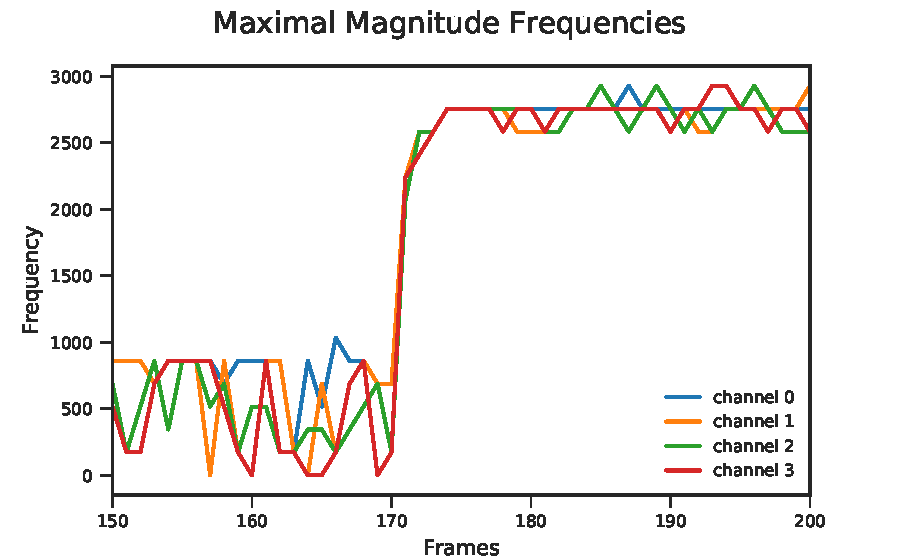
\includegraphics[]{figures/maxFreq}
	\caption{Frequencies of maximum magnitude in signal spectrum per frame.}
    \label{fig:03_maxFreq}
\end{figure}
% -------------------------------------------------------------
